%!TEX TS-program = xelatex

\documentclass[11pt,oneside]{book}
\usepackage[english]{babel}
\usepackage{uis-thesis}
\usepackage{listings}
\renewcommand{\lstlistingname}{Code}
\usepackage{listings-golang} % import this package after listings
\usepackage{color}

\definecolor{backcolour}{rgb}{0.95,0.95,0.92}

\lstset{
    backgroundcolor=\color{backcolour},
    basicstyle=\ttfamily\scriptsize,
    keywordstyle=\color{blue},
    stringstyle=\color{brown},
    numbers=left,
    numbersep=5pt,
    showstringspaces=false, 
    tabsize=4,
    captionpos=b,
    breaklines,
}
\newgeometry{margin=40mm}     % defines the geometry for the document
\setstretch{1.2}              % defines the default line spacing for the document
\setlength{\parindent}{0pt}
\setlength{\parskip}{\baselineskip}

% UiS recommends Georgia for the body text, but you are free to use another
% font for the body text; if you want to use another font just remove this line.
\setmainfont{Georgia}

%-----------------------------------------------------------------
\title{Quickfeed Support for Feedback via Pull Requests and Issues}
\authors{Ole Jørgen Espeland}
\department{ide}
\photo{photos/ide}
\photocredit{Ole Jørgen Espeland}
\reporttype{bachelor}
\specialization{cs}
% Uncomment only if your thesis has been granted restricted access
% \restricted

%-----------------------------------------------------------------
\begin{document}
\uiscover{4}                  % pick color scheme 1-9
\frontmatter
\pagestyle{empty}
\declaration
%!TEX root = ../thesis.tex

\abstract

QuickFeed is an automatic evaluation system, developed at the University of Stavanger.
Designed with the intent of easing assignment submissions, QuickFeed tests student code as they push it to a supported source control management system.
Based on the results of these tests, QuickFeed publishes feedback to students via its custom web interface.

In this thesis, we explore the possibility of further expanding how students receive feedback on their submissions, by using GitHub's pull request and issue features.

%!TEX root = ../thesis.tex

\acknowledgements

I would like to thank my supervisors for their enthusiasm and help with writing this thesis. 


\tableofcontents

% \input{frontmatter/abbrev}
% \input{frontmatter/symbols}

%-----------------------------------------------------------------
\mainmatter	  % Begin normal, numeric (1,2,3...) page numbering

% Include the chapters of the thesis, as separate files
% Just uncomment the lines as you write the chapters

%!TEX root = ../thesis.tex

\chapter{Introduction}
\label{ch:intro}

The University of Stavanger has for the last couple of years been developing a project known as QuickFeed.
Since its inception in 2015 \cite{autograder}, both teachers and students have contributed to its development. % (ref)

QuickFeed aims to ease the process of submitting student assignments for both students and the teaching staff.
Though not exclusively, the project is primarily developed with the intent of handling code based assignments.
QuickFeed will run predetermined tests on submitted code, and will use their results to provide feedback for students via its web interface.
Using QuickFeed, assignments can be both scored and graded without the teaching staff ever having to intervene.

To accommodate these features, QuickFeed uses GitHub to, amongst other things, manage student code.
GitHub is therefore one of the primary sites students interact with, when working on QuickFeed managed assignments.
Because of this, there is a desire to further integrate QuickFeed with GitHub.
Specifically, we aim to use GitHub's pull request and issue features to give students another avenue for manual and automatic feedback.

\section{Motivation and Background}
\label{sec:motivation}

In the current iteration of QuickFeed, students only receive automated feedback on their code through QuickFeed's custom web interface.
Here, they can see what parts of their code is failing, and also whether they have successfully passed the assignment.
The motivation behind this thesis is to further expand on how students receive feedback when working on an assignment.

Using GitHub pull requests we can facilitate manual feedback directly on student code by using its review features.
Pull requests also have the potential to support automatic feedback, e.g. by another GitHub feature called workflows.

\section{Objectives}

This project has the two following objectives.

To provide automated and manual feedback on student code, QuickFeed will support using GitHub pull requests.
Facilitating manual feedback means QuickFeed will decide when to assign reviewers to a pull request and who to assign.
When a pull request is approved, QuickFeed will also determine if this approval was legitimate.
To support automated feedback via pull requests, we want to use GitHub workflows, and have them work in conjunction with QuickFeed.

To further accommodate pull requests, we want QuickFeed to support task markdown files within an assignment.
These will function as a way for teachers to subdivide their assignment into smaller parts.
For each task, a GitHub issue will be created on every student repository by QuickFeed.
These issues are the ones students will base their pull request on.

\section{Approach and Contributions}

\begin{itemize}
\item Give a brief summary of your overall approach.
\item Summarize the specific contributions that you made in this thesis (implementation, empirical results, analysis, etc.).
\item It might be presented as a bullet list.
\end{itemize}


\section{Outline}

\begin{itemize}
\item Give an overview of the main points and the structure of your thesis.
\item Examples: ``Chapter 2 covers ...  Chapter 3 describes ...''
\item Show how the different parts (chapters) relate to each other.
\end{itemize}

% !TEX root = ../thesis.tex

\chapter{Background}
\label{ch:background}

In this chapter we describe existing technology and concepts that will be referred to throughout the thesis.

\section{GitHub}

QuickFeed already relies on GitHub to manage assignments and student code.
This section looks at certain GitHub features that we want QuickFeed to support.

\subsection{Issues}

GitHub issues is a useful feature for tracking, discussing and logging various issues/problems on a GitHub repository.
Any collaborator to a repository may open a GitHub issue, and describe any problem, idea or issue they have.
Other users may then contribute to the issue by commenting on it; thus easing the communication process within a project.
GitHub issues can therefore function as a discussion hub, and makes it especially useful for larger projects involving several people. 

\begin{figure}[ht]
    \centering
    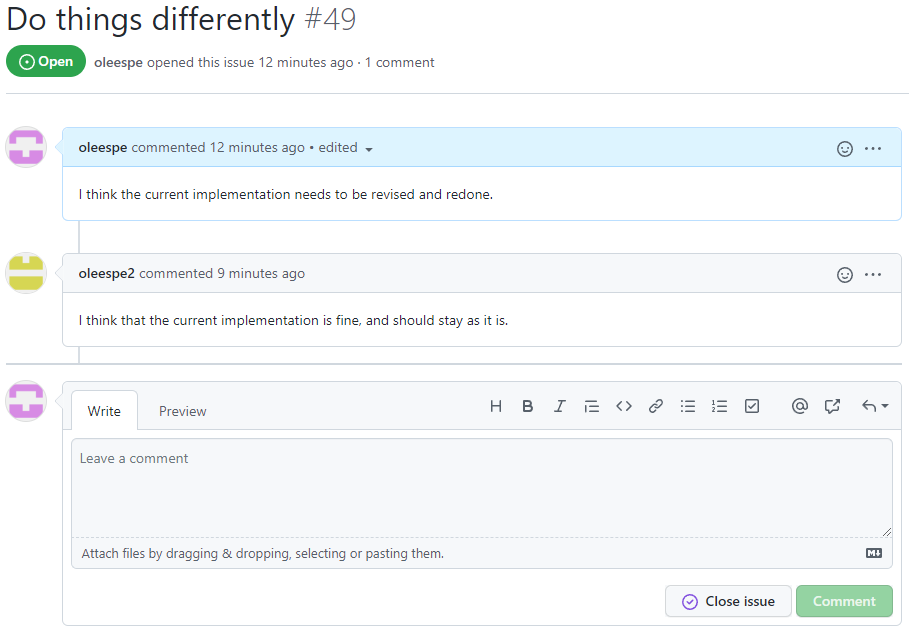
\includegraphics[width=\textwidth]{photos/github-issue.PNG}
    \caption{Example of a GitHub issue comment section}
    \label{fig:github-issue}
\end{figure}

\subsection{Pull Requests}

Pull requests are a desire to merge any feature branch, into the main branch of a git repository.
GitHub supports managing pull requests through its user interface, and allows any contributor to a repository to create a pull request.
Through the user interface, progress on a branch can be tracked, reviewed and commented on.
In this sense, GitHub pull requests function as a central hub for feature branches.

Code review is also a central part of the pull request process.
Any eligible user may review, comment on, and request changes to the source code of a given pull request.
The reviewer may also use reviews to approve a pull request for merging.

Pull requests can also be linked to issues.
Doing this will automatically associate any linked issue to the pull request, and cause them to close when the pull request closes.
A common workflow would be to create an issue, describing a problem, and then creating an associated pull request for this issue.

Through its features, GitHub pull requests provide an efficient and manageable way of implementing new features to any project.

\begin{figure}[ht]
    \centering
    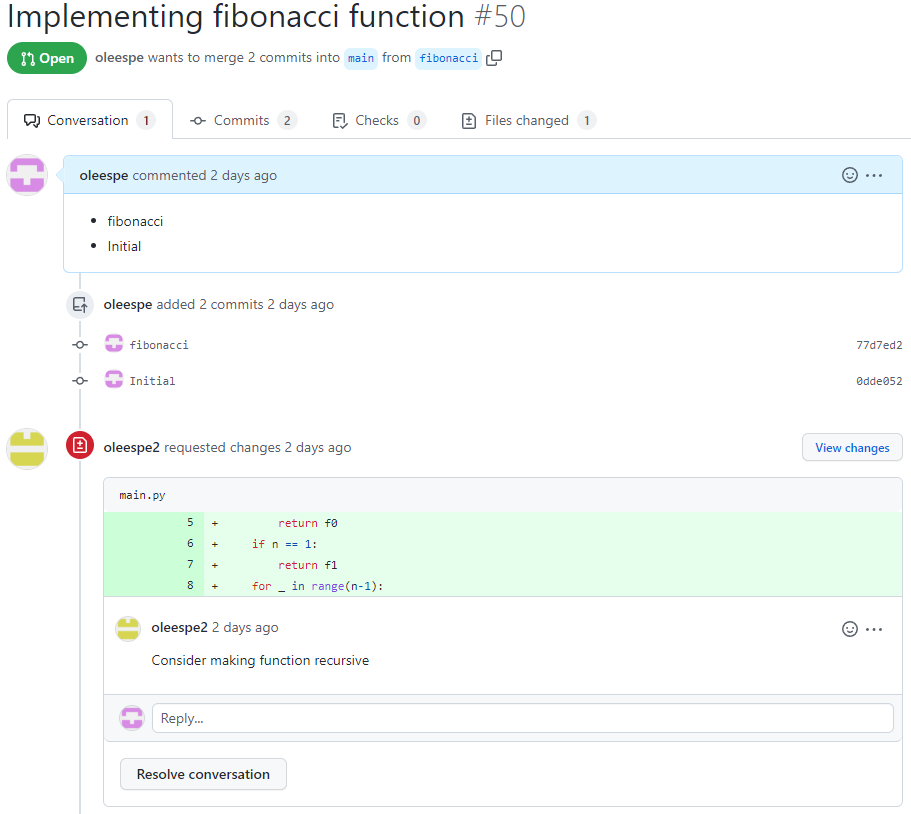
\includegraphics[width=\textwidth]{photos/pull-request.PNG}
    \caption{Example of a GitHub pull request}
    \label{fig:pull-request}
\end{figure}

\subsection{Workflows}

Maybe maybe

\section{QuickFeed}

QuickFeed provides two primary features.
A web interface that allows students to enroll in courses, create groups and receive feedback on their submissions.
And a backend that tests, scores and grades student submitted code.
The backend is primarily implemented with the Go programming language, while the frontend uses TypeScript and the React library.
For data storage, QuickFeed relies on an SqLite-database, managed using the the GORM library.
% TODO: Should consider splitting this chapter in two. One describing some of the technology QuickFeed uses, and one that highlights some of its % features

In this section we further describe some of QuickFeed's key concepts, as well as the technology it uses.

\subsection{Protocol Buffers}

Protocol buffers is a language-neutral mechanism for serializing structured data. % (ref: https://developers.google.com/protocol-buffers)
It is often abbreviated as protobuf, and is used to define messages in a \textit{.proto} file.
When the file is compiled, data structures and methods for the desired language are generated in a separate file.
QuickFeed uses protobuf to generate most of its data structures.
These are then stored in its internal database when necessary.

\begin{lstlisting}[caption={Group message}]
message Group {
    enum GroupStatus {
        PENDING  = 0;
        APPROVED = 1;
    }
    uint64 ID          = 1;
    string name        = 2;
    uint64 courseID    = 3;
    uint64 teamID      = 4;
    GroupStatus status = 5;

    repeated User users             = 6;
    repeated Enrollment enrollments = 7;
}
\end{lstlisting}

The code above is an example of such a message.
It holds a reference to a single \textit{Course} message and several \textit{User} messages, as seen on Line 8 and 12 respectively.
When compiled, the resulting data structure is used by QuickFeed to represent groups.

It should be noted that QuickFeed also uses all these messages in conjunction with gRPC to facilitate server-client communication.
This part is however not relevant for this project.

\subsection{QuickFeed Repository Structure}
\label{sec:quickfeed-repository-structure}

When a teacher creates a course in QuickFeed, a GitHub organization is created to represent it.
Within this organization, three initial repositories are created, as well as student repositories when students enroll.
They are all described as follows.

\textit{info}: This repository simply holds information about a course.
The repository is available to all students, and would typically work as a simple information hub.
It is created and managed by the teaching staff.

\textit{assignments}: The repository responsible for presenting the assignments to students.
Every assignment in a course is represented as a unique folder within this repository.
As teachers push new assignments to this repository, or update existing ones, students pull the changes to their own local git repositories.

\textit{tests}: Teachers use this repository to store both test code and files needed to facilitate automatic testing of student code.
It's folder structure should be one-to-one with \textit{assignments}, with every assignment being represented by a unique folder.
As students submit code for an assignment, QuickFeed tests it with all code from the folder representing that assignment.
In addition, the repository contains assignment specific \textit{assignment.yml} files, as well as a \textit{scripts} folder.
The \textit{scripts} folder is used to store a \textit{run.sh} file and a Dockerfile.

The \textit{assignment.yml} file is used by teachers to specify assignment specific settings.
As an example, it can contain information about the assignment deadline, whether it is manually graded, and more.

The \textit{run.sh} file contains the script used by QuickFeed when testing student code.
As explained, it is contained within the \textit{scripts} folder, but can also be located within the specific assignments themselves.
When running tests on an assignment, QuickFeed will prioritize using any assignment specific script files.

Finally, the Dockerfile contained within \textit{scripts} is used to create a docker image.
Within this image, QuickFeed runs the appropriate script, derived from \textit{run.sh}.

Being a repository that is used and managed solely by the teaching staff, it follows that students do not have access to its contents.

\begin{figure}[ht]
    \centering
    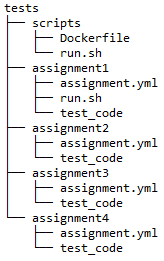
\includegraphics[scale=0.8]{photos/tests-repository-structure.PNG}
    \caption{Example of a tests repository folder structure}
    \label{fig:tests-repository-structure}
\end{figure}

Student repositories: There are two types of student repositories, user and group repositories.
A user in this case would simply be any student who has enrolled in the course.
Whereas a group is any number of students that are working together.
Naturally, student repositories are only accessible by the students associated with them, and the teaching staff.

Student repositories are named according to the following format: \textit{name-labs}.
For an enrolled student, \textit{name} would be their GitHub user name.
A group's \textit{name} however, would be defined by the group members themselves when they enroll the group.

These repositories are the ones students push their code to as they work on assignments.

\begin{figure}[ht]
    \centering
    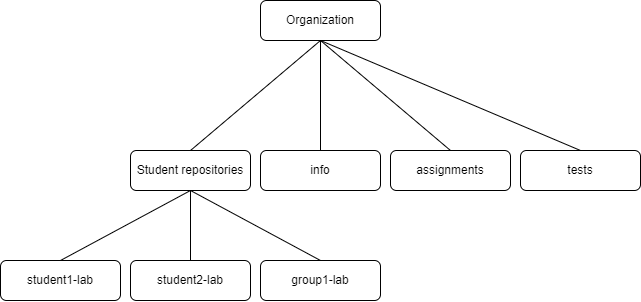
\includegraphics[width=\textwidth]{photos/qf-repository-structure.png}
    \caption{GitHub repository structure for a QuickFeed course}
    \label{fig:qf-repository-structure}
\end{figure}

\subsection{The Score Package}
\label{sec:the-score-package}

QuickFeed's score package allows for scoring student submitted code.
Every time a student pushes code to their repository, QuickFeed will run tests on the code, and generate a total score ranging from 0 to 100.
In this section we describe the parts of this package that are relevant for this thesis.

When teachers develop and push assignments to \textit{tests}, they also create test code that is meant to test student submitted code.
As part of the score package, teachers can specify for individual tests, what score they should give, and how that score is gained.
For example, a test can loop through several test conditions, and then decrement the score every time it fails.
These tests have to be explicitly added by teachers using either of the following methods: Add and AddSub.
Doing so, they are included in the pool of all tests that constitute an assignment.

Each individual score is defined in a data structure generated by the below protobuf message.

% TODO: Should maybe explain some of these fields
\begin{lstlisting}[caption={Score message}]
message Score {
    uint64 ID =           1;
    uint64 SubmissionID = 2;
    string Secret =       3;
    string TestName =     4;
    int32 Score =         6;
    int32 MaxScore =      7;
    int32 Weight =        8;
}
\end{lstlisting}

When QuickFeed is finished running all tests, a test results data object is extracted containing a list of all these scores.
These are then used to generate a total score for the submission in question.

\subsection{Testing Assignments}

Having explored how QuickFeed scores student code, this section will further explore parts of the assignment submission process that are important.

As students push code to their GitHub repository, QuickFeed will do two things.
First it will determine the assignments that have been changed since the last push.
Then, for every changed assignment, it will run the tests defined for that assignment in \textit{tests}.

Running the tests uses QuickFeed's ci package.
To set up a test environment, QuickFeed uses the Dockerfile found in \textit{tests} to create a docker container.
It then continues by running the assignment's script file, as mentioned in Section \ref{sec:quickfeed-repository-structure}.
These script files can be assignment specific, but generally they use git clone to merge the students code with the assignment tests, followed up by a command to run all tests.
The ci package also supports supplying the script with arguments, e.g. to clone the correct student repository.

When this process is finished, QuickFeed extracts the test run's results and uses them to determine whether the student got a passing score.

\subsection{Webhooks}
\label{sec:webhooks}

QuickFeed communicates with GitHub in two ways.
In this section we will detail one of them, namely webhooks.

A webhook is a "user-defined callback over HTTP". % (ref: (09.04) https://developer.atlassian.com/server/jira/platform/webhooks/)
In general, webhooks allow developers to listen to events from any supporting site.
When any such event occurs, an HTTP request is sent to the address configured for the webhook.
The request contains data about the event, usually in a JSON format.

QuickFeed uses webhooks to retrieve data from push events on a course.
When a new course is created, QuickFeed creates a webhook on the GitHub organization of the given course.
This webhook is only triggered by push events, which are then handled by QuickFeed accordingly:

\begin{itemize}
    \item If a push event is associated with the \textit{tests} repository, QuickFeed will update the course assignments.
    \item If a push event is associated with a student repository, QuickFeed will determine the assignments that have been changed/worked on, 
    and run the assignment tests on them.
\end{itemize}

\subsection{Source Control Management API}
% TODO: Should say that QF authenticates with the GitHub API by being an Oath app.
The second way QuickFeed communicates with GitHub is through a custom API.

To facilitate communication with potentially any source control management system, a custom API has been developed for QuickFeed, which is usually abbreviated as the SCM API.
The current iteration of QuickFeed supports interacting with GitHub through this API, via the go-github library. % (ref: go-github)
The library itself, communicates with GitHub's own REST API using HTTP requests.

The SCM API allows QuickFeed to perform various tasks, such as creating/updating repositories, creating webhooks, managing teams and more.
QuickFeed's SCM API, together with webhooks, form a 2-way communication stream between QuickFeed and GitHub.
%!TEX root = ../thesis.tex

\chapter{Related Work}
\label{ch:related}

Should at least mention Adil's report here.
%!TEX root = ../thesis.tex

\chapter{Approach}
\label{ch:approach}

Before we can start implementing anything, there are a few lingering design choices we have to make.
In this chapter we discuss and analyse these, and try to give a rationale for why we made the choices that we did.
% TODO: Hein recommends a recap of the goals of the project somewhere here

\section{Student Repository Access}

Since students do not have access to other students' repositories, they have no easy way of accessing their code.
This becomes a necessity when want to do co-student code review, as they must somehow be given access to the relevant pull request.
In this section we discuss possible solutions to overcome this problem.

\subsection{Possible Solutions}

A solution could be to use GitHub teams, a feature that would allow us to grant limited access to individual repositories.
When a student is assigned to review someone else's pull request, such a team can be created with read rights to the relevant repository.
Once the review is finished, we can either remove the team from the repository, remove the student from the team, or just delete the team altogether.
This solution does however have some unwanted side effects, which can be illustrated with the following scenario.

Imagine we have two students: A and B.
Student A is finished with a task from assignment 1, and therefore gets a reviewer assigned.
Student B is assigned to review it, and is granted access by QuickFeed to student A's repository.
Student A is also diligent, and has already started working on assignment 2.
In fact, student A has nearly completed assignment 2.
Student B however, has not even started on assignment 2, but because they can now access student A's assignments, they see how he/she did it.

As a consequence, using GitHub teams would mean that assignments can only be published after the deadline of the previous one is passed.
A prospect that would probably not be appealing to most teachers.

Another possible solution is to create a clone repository, containing only the relevant assignment. 
This way, any reviewing student will only have access to the assignment in question.
QuickFeed would create these repositories when needed, and then delete them once the review is complete.

Implementing this however seems highly complex, as there is a myriad of complications and problems that will have to be accounted for.
For one, QuickFeed must be expanded to handle, amongst other things, the following.

\begin{itemize}
    \item Creating clone repositories containing only the assignment that is relevant, and the accompanying pull request.
    \item Deleting these repositories when they are no longer needed.
    \item Associating actions on the original repository with the new one.
    I.e., we must make sure that any relevant additions to the original repository are reflected in the cloned one.
    \item Account for all possible complications that may occur.
\end{itemize}

An implementation like this also assumes that only one review is required per assignment, when there could in fact be several.
If for example an assignment has three tasks, and therefore three related pull requests, how do we then create these clone repositories?
Would we create one per pull request?
This seems like a terrible approach, as the number of repositories created would me enormous in courses with many students.

Let us say that we, despite these challenges, managed to create a fully functional implementation of the above solution.
We now have to cope with the prospect of having further complexified the user experience.
Possibly so much so that the entire solution might be counter-productive.

\subsection{Limiting Scope to Group Repositories}

The two solutions proposed in the previous section either seem too complex, or somewhat suboptimal.
Instead of going through with one of them, a compromise was agreed on to limit the project scope to only group assignments.
This means that instead of students reviewing each other's code on regular assignments, they will only do so on group assignments.
Furthermore, students will also only review other group members' code.

As an example, we can imagine a group assignment with three different tasks.
A group of three students will create a pull request each to solve these tasks.
They are then each assigned, when appropriate, to review one of the other group members' pull request.

The benefit of this approach is that it avoids students needing access to other repositories all together.
We only need to manage student review within a local group scope, and not for an entire course.

One disadvantage is that teachers will have to more carefully plan out the tasks they create.
Say we have a group of four members, and a group repository with only three issues.
One of the issues will have to be shared by two of the group members.
If every issue is equally challenging to solve, it would put the other two members at a disadvantage.
It seems then that teachers should only create as many tasks as there are designated group members, or at least a multiple of that number.

Another consideration teachers will have to account for, is that they have to create tasks that are independent of each other.
If task A is dependent on task B being complete, a consequence would be group members potentially having to wait for each other.

\section{Creating Pull Requests}
\label{sec:creating-pull-requests}

Having limited our approach to only group assignments in the previous section, we continue by discussing how to create the pull requests themselves.

There are two viable options, both with their own set of advantages and disadvantages.
Option one is to have students create the pull requests.
As issues are created on their group repository, the group members can internally decide who solves what issue.
Option two is having QuickFeed create the individual pull requests when tasks are created.

\subsection{Manual Creation}

An advantage of letting students manually create the pull requests, is that group members can self organize on who does what.
If a group member thinks a certain issue looks more interesting than the others, they can explicitly communicate this with the rest of the group.

Manually creating a pull request also allow us to restore a working state, in case a student incorrectly merges it.
This could happen if the pull request has not been approved by a teacher.
The same process we use internally to create the pull request, can be used again to recreate it.

The major disadvantage to relying on students to create the pull requests, is the increased complexity that comes with it.
Students will have to learn how to create and merge them correctly, and when to do so.
If a student messes up, they must know how to fix any potential complications.
And if they do not, the teaching staff must have the capacity to assist them.

\subsection{Automatic Creation}

The clear advantage to having QuickFeed automatically create pull requests, is that we do not make the process more complex for students.
If the students are not involved, there is no opportunity for them to mess up.
This also alleviates the teachers, as they no longer need to assist in case something goes wrong.

There is however a disadvantage to this approach.
Given that QuickFeed relies on authenticating with GitHub using users specific access tokens, each pull request would have to be made either in a student or teacher's name.
Both of these options seem suboptimal.
Creating them as teachers seems illogical, as one teacher will then be the owner of a huge number of pull requests they do not interact with.
If we create them as students, we could do so for each individual group member.
This still leaves us with the issue of having to decide what group member to use when creating the pull request
If the number of issues in a repository does not align with the number of group members, what should happen?
Even if we solve these problems, we are still left with the fact that individual group members can no longer self organize when assigning issues.

It seems then that any solution must create "anonymous" pull requests, i.e pull requests that are not directly assigned to any student or teacher.
One way to do this could be to have a QuickFeed bot account.
This bot account would then be the user used to create all required pull requests 
There are however drawbacks to this approach as well.
To facilitate student co-review, we must have a reference to the student who "checked out" the pull request.
If we do not, we will have no way of knowing from which pool of group members to select a reviewer later on.
This is given the fact that a student should not be assigned to review their own pull request.

\subsection{Conclusion}

While option two seems ideal, there are a few key points that made us instead go with option one.
First of all, the current iteration of QuickFeed does not seem to fully support it, as we have no direct way to create anonymous pull requests.
Secondly, option one gives us a greater capacity to handle students incorrectly mergeing pull requests.

It is worth noting that these two approaches are not mutually exclusive, and QuickFeed could support both solutions at the same time.
In fact, the initial idea was to implement them both, and thus getting all their benefits.

\section{Issue Creation}

Having discussed our approach on creating pull requests, we continue by exploring a similar problem.
How do we create issues?

As mentioned previously, we want to create issues on every group repository in a course.
To create these issues, we must use the GitHub API.
And again, given that GitHub authenticates on a per user basis, these issues must be created in the name of either a student or teacher.

Like with the pull request problem, creating them as a teacher seems wrong, however, creating issues as a student does not seem that problematic.
It does not matter, given our context, who is assigned as an issue owner.
The issues only serve as a source of information, and the only time students interact with them is when they create pull requests.

A solution could then be to simply have the first student within a group be set as the issue creator.
Of course, this is a somewhat "hacky" solution, as it makes more logical sense to have QuickFeed assigned as the owner.
Which again boils down to the fundamental issue on how QuickFeed authenticates with GitHub.

\section{Automated Student Feedback}

To facilitate automatic feedback on individual pull requests, the initial idea was to use GitHub workflows.
Mainly due to the fact that workflows are already tightly integrated into the GitHub pull request user interface.

As students work on tasks, we imagined using workflows to give feedback based on the tests run on their code.
However, as we researched ways to implement this, it became apparent that workflows were not an optimal approach.
For one, to have GitHub register a workflow, a \textit{.yml} file describing it must be present on the repository.
These files would have to be created and pushed to \textit{tests}, and then pulled by every student.
The biggest problem however, is that GitHub does not support triggering workflows manually via API, and at the same time having them appear in a pull request.
Meaning that we can trigger workflows remotely, but we cannot have them be displayed within a pull request on the same trigger.

As a consequence we have to find potential alternate solutions.
These are discussed in detail in the following sections.

\subsection{Pull Request Comments}

Instead of providing automatic feedback via GitHub workflows, we can instead do so by commenting on the pull request itself.
GitHub's API allows for doing this, again with the caveat that we must comment in a student or teachers name.
Here, the easiest solution is to simply comment as the student that created the pull request.

\subsection{GitHub Checks API}

Another interesting option is to use GitHub's Checks API.

Cannot use because not GitHub App
Must explore this further before describing it.

\section{Feedback content}

Not fully implemented yet.
Also what should this feedback consist of? Can look at the type of automatic feedback they receive in web interface.

\section{GitHub App}

Should discuss the need to be able identify as QuickFeed when performing many of the actions needed in the implementation.
These include creating issues, creating pull requests and if 
%!TEX root = ../thesis.tex

\chapter{Implementation}
\label{ch:implementation}

Text text

\section{Existing implementation}

As we have already mentioned, an implementation has already been attempted for this project.
Before we can begin with a new one, we first have to decide which parts of the existing one we want to use, and which to discard.
These parts are summarized in this section.

\subsection{SCM Expansion}

The SCM package has been expanded for GitHub to support the following functions:

\begin{itemize}
    \item CreateIssue   - creates an issue on a repository.
    \item EditRepoIssue - edits an issue on a repository.
    \item GetRepoIssue  - retrieves an issue based on issue number and repository.
    \item GetRepoIssues - retrieves all issues from a repository.
\end{itemize}

CreateIssue and EditRepoIssue would prove useful, and are used with only minor adjustments to them.
The two other functions, centered around retrieving issues were not needed, but still used in earlier parts of the project when testing.

\subsection{Logic}

A lot of existing code was intended to handle the logic around managing tasks. 
In short, this code was meant to do determine when to create, edit or delete issues on GitHub.
The code did however not accomplish this in a functional manner.
This lead to the dilemma of whether we should continue developing this faulty code, or simply start anew.
In the end, it was decided that any attempt to fix the existing logic code would be more time consuming and confusing, than simply starting fresh.

\subsection{Parsing Tasks}
\label{sec:parsing_tasks}

When a teacher pushes assignments to the \textit{tests} repository QuickFeed will run the function UpdateFromTestsRepo.
In short, this function fetches the files of \textit{tests}, loops through them, and uses their contents to create or update the data records of all course assignments.
Added as a part of this process, was code to also fetch task files in the repository, and use their contents to create a task data object.

To support this, all \textit{task-*.md} files are expected to conform to a standard format.
The first line should start with the character sequence "\# <task title>", followed by by two new line characters.
Any following text will be treated as the task body or description.

Using this format, the function newTask creates a task data object from any task file.

\lstinputlisting[caption={Function that creates a task object from markdown content}, language=Golang, firstline=25, lastline=40]{code/tasks.go}

Going forward, the general approach to parsing and creating tasks is left as it is, with only minor changes to the existing code.

\section{Managing Tasks and Issues}

Having looked at what existing code we decided to keep, we continue by exploring the part of the project that was implemented first, how to manage tasks and issues.
Building on what is described in section \ref{sec:tasks_and_github_issues}, this section describes the actual implementation process.

Moving forward in this chapter, we make the following distinction between found tasks and assignments, and existing tasks and assignments.
Found tasks and assignments are data objects created from the contents within the \textit{tests} repository.
Existing tasks and assignments are data-objects based on data records that we retrieve from the database.

\subsection{Data structures}

Two new messages are defined in the ag.proto file: \textbf{Task} and \textbf{Issue}.
These are used to generate the data structures that we use throughout the rest of the project.

\textbf{Task} is defined as follows:

\lstinputlisting[caption={Task message}, firstline=185, lastline=193]{code/ag.proto}

Every task is associated with one assignment via the \textit{assignmentID} field.

For assignments, \textit{order} is a number used to determine the order in which assignments are represented in a course.
Tracking the order of the assignment a task came from, allows us to associate tasks and assignments without explicitly knowing the assignment ID, so long as our scope is limited to just a single course.
A feature that will prove necessary.

The \textit{name} field is used to associate tasks found on GitHub, with the ones stored in the database.
If a task file with the name task-hello\_world.md is found within assignment1, then its corresponding name will be assignment1/hello\_world.
This name is set when the task itself is parsed, as described in section \ref{sec:parsing_tasks}.

\textbf{Issue} is defined as follows:

\lstinputlisting[caption={Issue message}, firstline=195, lastline=200]{code/ag.proto}

We see that every issue holds an association to the task that was used to create it, as well as the repository it was created on.

The \textit{issueNumber} field represents the issue number GitHub will assign the issue on its creation.

As it will become important in the next section, we will also mention that a modification was made to the existing message \textbf{Assignment}.

\lstinputlisting[caption={Assignment message}, firstline=168, lastline=183]{code/ag.proto}

On line 14 on the above code we see that the message has repeated tasks.
When we compile it, the resulting data structure can hold a slice of tasks.

\subsection{Main Logic}

As mentioned in section \ref{sec:parsing_tasks}, UpdateFromTestsRepo is the function that is run when someone pushes to the \textit{tests} repository.
Since tasks and issues need to be synchronized every time this happens, all logic for doing so will happen here.

More specifically, we create the function handleTasks that handles all logic relating to tasks.
It is supplied with every found assignment, and their respective found tasks, as an argument.
The function itself is run at the end of UpdateFromTestsRepo.

\lstinputlisting[caption={The function handleTasks, responsible for all task related logic}, language=Golang, firstline=64, lastline=95]{code/tasks.go}

The logic contained in this function will be explained in the following sections.

\subsection{Synchronizing Tasks}

When teachers create, edit, and delete tasks, we must make sure that the same happens in QuickFeed's internal database.
To accomplish this, we created the database method SynchronizeAssignmentTasks to synchronize tasks correctly.
This method is run at the start of handleTasks, and can be summarized in the following chart.

\begin{figure}[ht]
    \centering
    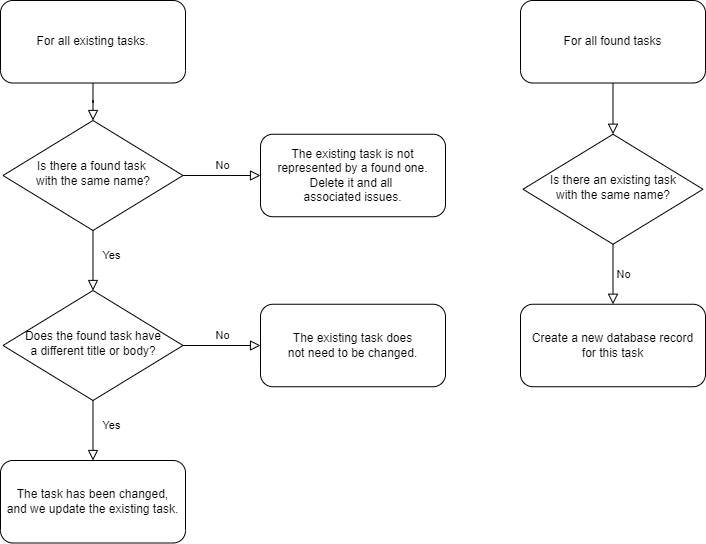
\includegraphics[width=\textwidth]{photos/synchronize-tasks-flow-chart.png}
    \caption{Flow chart describing how tasks are synchronized}
    \label{fig:synchronize-tasks-flow-chart}
\end{figure}

To support this logic, SynchronizeAssignmentTasks utilizes Go's built in maps to map tasks by both assignment order and name.
When looping through all existing assignments and then their respective existing tasks, we can use this mapping to perform all checks described in the chart above.

\lstinputlisting[caption={Logic performed in SynchronizeAssignmentTasks}, language=Golang, firstline=41, lastline=76]{code/gormdb_tasks.go}

SynchronizeAssignmentTasks also returns the tasks it has created or updated, which will be important when synchronizing issues.

\subsection{Synchronizing Issues}

\section{Tests}

Maybe maybe
%!TEX root = ../thesis.tex

\chapter{Discussion}
\label{ch:discussion}

There is nothing stopping a student to ignore everything we have done, and simply solve an assignment manually.
I.e, there is nothing enforcing a PR review.

What happens if a teacher creates two tasks with the same name?

There is a weakness in how we handle branches.
If someone pushes to a branch with a remote name that differs from the local name, we cannot know which local branch to check out.

The issue and task related code can easily be extended to also work on all student repositories.
The pull request part is more hard coded.
Can discuss any potential expansion to make it also work on regular student repositories.

Can maybe discuss the potential to have a more efficient way of testing things, such as webhook related stuff.
For example, I am currently hard coded into some of the db population functions, to facilitate testing.
Would be better if this was more independent. 
Could maybe have certain QF test GitHub users?

Should discuss that finding the linked issue by parsing the PR body limits what can be in it.
Can maybe instead be implemented as a regular expression search.

\section{Future Work}

Maybe more feedback if students do something wrong.
For example, if a student creates a pull request without correctly linking the issue, they should probably be immediately made aware.
In this case, we could maybe comment on their pull request, stating this.
We could also support students linking issues late by listening to pull request body changed events, or something.
This avoids the need for students to recreate pull requests in case they fail.

\subsection{Checks API}

\subsection{Expanding Approval Process}
Pull requests can be approved. This has no impact on the assignment approval process. Can expand on it.

\subsection{GitHub App}
\label{section:github-app}

QF should probably be a GitHub app instead of Oauth app
Oauth app acts on behalf of a user, while app uses its own identity.
For example, with an Oauth app we cannot create pull requests and comments as QF, only as an authorized user in that org.
All issues that are created will be in the course creators name.
Also required for Checks API.
https://docs.github.com/en/developers/apps/getting-started-with-apps/differences-between-github-apps-and-oauth-apps
https://docs.github.com/en/developers/apps/getting-started-with-apps/about-apps

%!TEX root = ../thesis.tex

\chapter{Conclusions}
\label{ch:conclusion}



%-----------------------------------------------------------------
% Now begin the Appendices, including them as separate files

% \listoffigures
% \listoftables

\appendix

%-----------------------------------------------------------------
% \backmatter

% \label{Bibliography}
% \lhead{\emph{Bibliography}}  % Change the left side page header to "Bibliography"
% \bibliographystyle{unsrtnat}  % Use the "unsrtnat" BibTeX style for formatting the Bibliography
% \bibliography{Bibliography}  % The references (bibliography) information are stored in the file named "Bibliography.bib"

\uisbackcover
\end{document}
